\chapter{Detalii de implementare}

\section{Structura de directoare}

Aplicația, la nivelul cel mai înalt, are 3 module Python (interpretorul
Python directoarele ce conțin fișierul gol \texttt{\_\_init\_\_.py} ca
fiind module):
\begin{description}
\item [authentication] este modulul responsabil înregistrare și autentificarea
utilizatorilor. Acest modul conține modelul ORM al utilizatorului și
view-urile REST corespunzătoare creării de utilizatori noi și
autentificării unui utilizator.
\item [expenses] este modulul ce conține modelul ORM al unuei cheltuieli
și view-urile REST corespunzătoare operațiilor CRUD asupra
cheltuielilor.
\item [money\_keep] este modulul responsabil de configurarea aplicației.
Conține, printre altele, fișierul de configurare \texttt{settings.py}
și fișierul ce conține toate rutele aplicației (URL-urile la 
care aplicația răspunde), \texttt{urls.py}.
\end{description}

Pe lângă aceste module, la nivelul cel mai înalt al aplicației
mai sunt directoarele:

\begin{description}
\item [static] conține toate resursele statice: 
  \begin{itemize}
  \item componentele instalate cu \emph{Bower}
  \item CSS-urile customizate ale aplicației
  \item întreaga aplicație AngularJS, cu toate șabloanele,
  controllerele, directivele și serviciile ei.
  \end{itemize}
\item [templates] conține șabloanele Django. Ele sunt scrise
folosind sintaxa \emph{Django Template Language} (DTL) și nu trebuie confundate
cu șabloanele din directorul "static/templates". Șabloanele din
acest director sunt folosite de Django, iar cele din "static" sunt
folosite de AngularJS.
\end{description}

\begin{lstlisting}[title=Structura de directoare a aplicației]
|-- authentication
|   |--- migrations
|-- expenses
|   |--- migrations
|-- money_keep
|-- static
|   |-- bower_components
|   |-- css
|   |-- js
|   |   |-- authentication
|   |   |   |-- controllers
|   |   |   |--- services
|   |   |-- expenses
|   |   |   |-- controllers
|   |   |   |-- directives
|   |   |   |--- services
|   |   |-- layout
|   |   |   |--- controllers
|   |   |--- utils
|   |       |-- controllers
|   |       |--- services
|   |--- templates
|       |-- authentication
|       |-- expenses
|       |-- layout
|       |--- utils
|--- templates
\end{lstlisting}


\section{Module AngularJS}

Pe partea de front-end, aplicația este structurată
în următoarele module:
\begin{description}
\item [authentication] este modulul responsabil de autentificare.
Acest modul conține serviciul \emph{Authentication} care are metodele
pentru autentificare, logout și verificarea dacă utilizatorul este
autentificat.
\item [expenses] este modulul responsabil de operațiile
CRUD pentru o cheltuială. Pe lângă serviciul care are apelează
metodele REST ale back-end-ului, în acest modul sunt definite și directivele
AngularJS \emph{expense} și \emph{expenses}. Aceste directive
fac posibilă folosirea în șabloane AngularJS a elementelor HTML
\texttt{<expense>} și \texttt{<expenses>}.
\item [layout] este modulul care conține logica de filtrare / căutare
a cheltuielilor și leagă butoanele din bara de navigare de funcționalitatea
acestora.
\item [utils] este un modul care conține logica de printare
precum și un serviciu utilitar ce se ocupă cu prelucrarea
obiectelor date / time.
\end{description} 

\section{API REST}

Deoarece front-end-ul aplicației este scris cu AngularJS,
comunicarea dintre front-end și back-end se face
prin intermediul unui API REST. Acest API REST a fost
creat cu ajutorul unui plugin Django: 
\emph{Django REST Framework}\footnote{\url{http://www.django-rest-framework.org}}.

Django REST Framework permite crearea rapidă de API-uri REST pentru 
aplicațiile Django. Pentru a îl folosi, în aplicație am creat
câte o clasă de serializare pentru fiecare model 
ce trebuie serializat (\texttt{Account} și \texttt{Expense}).
Aceste clase moștenesc din \texttt{rest\_framework.serializers.ModelSerializer}.
În clasele de serializare specificăm ce câmpuri vrem să fie serializate.
Clasele de serializare pot fi văzute în "authentication/serializers.py"
și "expenses/serializers.py".

În afară de clasele de serializare, am creat și permisiuni pentru fiecare
model. Folosindu-ne de aceste permisiuni, ne asigurăm că un utilizator
nu poate citi datele altui utilizator. Permisiunile se găsesc
în fișierele "permissions.py" din modulele "authentication" și
"expenses".

Având permisiunile și clasele de serializare, folosim clasele
din rest\_framework pentru a customiza mai departe
operațiile pe care le dorim: de exemplu pentru filtrarea 
cheltuielilor după dată, sau pentru a crea un utilizator nou
stocându-i parola în formă hash.

API-ul creat este următorul:
\begin{description}
\item [POST /api/v1/auth/login/] permite logarea unui
utilizator în aplicație. Parametrii primiți sunt
adresa de email a utilizatorului și parola.
\item [POST /api/v1/auth/logout/] deautentifică
utilizatorul curent.
\item [POST /api/v1/accounts/] crează un utilizator nou.
Primește ca parametri numele utilizatorului, parola
și adresa de email.
\item [GET api/v1/expenses/] întoarce lista cu toate
cheltuielile pentru utilizatorul logat în aplicație.
\item [POST /api/v1/expenses/] adaugă o cheltuială
nouă.
\item [DELETE api/v1/expenses/\{:id\}/] șterge cheltuiala
cu id-ul specificat.
\end{description}


\section{Fluxul aplicației}

Fiind o aplicație SPA ce folosește un framework MVC
pe back-end și un alt framework MVC pe front-end,
rutarea URL-urilor are loc la două nivele.

Orice request către aplicație este mai întâi redirecționat
de URL handler-ul Django. În fișierul \texttt{urls.py} sunt
configurate toate rutele aplicației. Indiferent ce pagină
cere utilizatorul, acestuia îi este servit șablonul Django
\texttt{index.html} ce conține întreaga aplicație AngularJS.

A doua rutare are loc la nivelul AngularJS. Serviciul de autentificare
din AngularJS verifică dacă utilizatorul este autentificat sau nu.
Dacă nu este, utilizatorul este redirectat către pagina de autentificare.
Este important să înțelegem că acest redirect se întâmplă
doar prin Ajax. AngularJS este cel care cere șablonul HTML
"login.html" de pe server și îl afișează pe client, fără ca pagina
să fie reîmprospătată.

\section{Autentificarea}

Django, prin structura sa modulară, include un modul de autentificare,
numit \texttt{auth}. Acest modul conține un model, numit \texttt{User}
ce poate fi folosit de aplicațiile Django pentru autentificare.
În cazult acestei aplicații, am decis să nu folosesc acest model,
ci să-mi creez propriul model, ce moștenește din \texttt{AbstractBaseUser},
model din care moștenește și clasa User.
În acest mod, am putut modifica logarea standard din Django, bazată
pe username, cu logarea bazată pe adresă de email.

\lstinputlisting[language=python, title=authentication/models.py]{./chap6-files/account.py}

Autentificarea este pe bază de cookie. Pe pagina de autentificare,
AngularJS face POST la endpoint-ul "api/v1/auth/login". Dacă
user-ul și parola se potrivesc, server-ul răspunde cu codul 200 (OK).
În acest caz AngularJS folosește serviciul \$cookies pentru a reține
datele de sesiune primite înapoi de la server. Acestea sunt trimise
până la logout cu fiecare request, astfel serverul știe
că utilizatorul s-a autentificat în aplicație.

Codul JavaScript ce se ocupă de autentificare este în directorul
"static/js/authentication". Aici se găsesc controllerele pentru login și
register și serviciul de autentificare. Șabloanele corespunzătoare
loginului și funcției de înregistrare utilizator nou sunt în directorul
"static/templates".

În fișierul \emph{authentication.service.js} este definit serviciul
AngularJS \emph{Authentication}. Acest serviciu are funcțiile:
\begin{description}
\item [register] primește ca parametri email-ul, username-ul și
parola. Cu acestea, face POST la endpoint-ul \emph{api/v1/accounts}.
Dacă răspunsul este 200 (OK), ceea ce înseamnă că backendul
a creat un utilizaor nou cu credențialele trimise,
serviciul cheamă funcția "login".
\item [login] ia ca parametrii emailul și parola, cu care
face post la endpoint-ul 'api/v1/auth/login'. Dacă răspunsul este
200 (OK) atunci este setat un cookie cu utilizatorul autentificat,
iar utilizatorului i se afișează pagina cu cheltuielile sale.
\item [isAuthenticated] verifică dacă a fost setat
un cookie cu utilizatorul curent. Returnează \texttt{true} dacă 
utilizatorul s-a autentificat sau \texttt{false} dacă utilizatorul
nu este autentificat.
\item [logout] face POST la endpoint-ul 'api/v1/auth/logout' care îi
spune server-ului să deautentifice utilizatorul curent. După POST 
funcția \texttt{unauthenticate()} este chemată.
\item [unauthenticate] șterge utilizatorul autentificat din cookie.
\end{description}

\lstinputlisting[language=Java, title=static/js/authentication/services/authentication.service.js]{./chap6-files/authentication.service.js}

În șabloanele HTML pentru înregistrarea utilizatorului nou și pentru
login se găsește câte un form. În momentul în care utilizatorul face
submit acestui form, este apelată o metodă din controller-ul corespunzător
(login sau register) care, la rândul său apelează metoda serviciului.

\begin{lstlisting}[language=html, title=static/templates/authentication/register.html]
<form role="form" ng-submit="vm.register()">
  <div class="form-group">
      <label for="email">Email</label>
      <input type="email" class="form-control" 
             id="email" ng-model="vm.email"
             placeholder="email" required="" />
  </div>
  <!-- ....... -->
\end{lstlisting}

Prin folosirea directivei "ng-submit", aplicația Angular știe
că în momentul în care se face submit form-ului, trebuie
chemată funcția "register()" din controller. Prin folosirea
directivelor "ng-model", frameworkul crează o legătură
bidirecțională între textul din elementele "input" HTML
și proprietățile controllerului. De exemplu, de fiecare
dată când valoarea inputului "email" se modifică,
proprietatea "email" este setată pe controller astfel încât
valoarea ei să reflecte valoarea inputului.


\section{Operații CRUD pentru Expense}

Pe partea de client, serviciul care se ocupă de operațiile
CRUD corespunzătoare unui cheltuieli se numește \emph{Expenses}
și se găsește în fișierul "static/js/expenses/services/expenses.service.js".

\lstinputlisting[title=static/js/expenses/services/expenses.service.js]{./chap6-files/expenses.service.js}

Acest serviciu are metodele:
\begin{description}
\item [all] este funcția care face un HTTP GET la enpoint-ul
"/api/v1/expenses/". Această funcție primește un parametru
opțional: \emph{week\_contains}, care este un obiect reprezentând
o dată. Dacă parametrul este specificat, acesta este trimis
ca parametru GET serverului. Serverul întoarce lista cu toate
cheltuielile utilizatorului, dacă parametrul "week\_contains"
nu este specificat, sau o listă cu aferente săptămânii
din care data din "week\_contains" face parte, dacă parametrul
este specificat. Funcția întoarce un 
\emph{Promise}\footnote{\url{http://www.html5rocks.com/en/tutorials/es6/promises/}}
care este îndeplinit în cazul în care serverul răspunde cu 200 (OK)
cu lista de cheltuieli returnate de server.
\item [create] este o funcție care primește ca parametru
un obiect ce conține detaliile unei cheltuieli (dată,
titlu, descriere, comentarii) și face un HTTP POST
la endpoint-ul "api/v1/expenses" cu aceste detalii.
Serverul crează o cheltuială nouă cu detaliile primite
și o asociază utilizatorului curent.
\item [update] este o funcție care primește, ca și create,
un obiect cu detaliile unei cheltuieli. Spre deosebire de
obiectul pe care-l primește create, în update obiectul
trebuie să aibe setat și atributul "id". Funcția face
HTTP PUT la endpoint-ul '/api/v1/expenses/{id}/',
unde '{id}' este înlocuit cu "expense.id". Ca urmare
a acestui apel, server-ul ia din baza de date 
cheltuiala cu ID-ul specificat în adresă și updatează
acea cheltuială.
\item [destroy] este metoda responsabilă cu ștergerea
unei cheltuieli. Această metodă funcționează ca și update,
cu diferența că metoda HTTP folosită este DELETE în loc
de PUT.
\end{description}

\lstinputlisting[language=python, title=expenses/views.py]{./chap6-files/expenses.py}

Toate aceste metode sunt folosite de controller-ele din
"static/js/expenses/controllers", și anume: "EditExpenseController",
"ExpenseController" și "NewExpenseController".

De asemenea, în "static/js/expenses/directives" avem definite două
directive, și anume: "expenses" și "expense".
Aceste directive permit folosirea elementelor HTML <expense>
și <expenses> și fac astfel codul mai modular și concis.

\lstinputlisting[title=static/js/expenses/expenses.directive.js]{./chap6-files/expenses.directive.js}
\lstinputlisting[title=static/js/expenses/expense.directive.js]{./chap6-files/expense.directive.js}
\lstinputlisting[language=html, title=static/templates/expenses/expenses.html]{./chap6-files/expenses.html}
\lstinputlisting[language=html, title=static/templates/expenses/expense.html]{./chap6-files/expense.html}


\section{Modulele "layout" și "utils"}

În "static/js/layout/controllers" avem două controllere:
\emph{IndexController} și \emph{NavbarController}.

IndexController "ascultă"
pe "\$scope" propagarea evenimentelor "expense.created", "expense.deleted"
și "expenses.filter", iar când unul din aceste evenimente este
declanșat, se face filtrarea cheltuielilor și variabila
"vm.expenses" este actualizată.

\lstinputlisting[title=static/js/layout/navbar.controller.js]{./chap6-files/navbar.controller.js}

NavbarController implementează funcțiile accesibile
din bara de navigație: logout, adăugare cheltuială nouă
și deschiderea dialogului cu selectarea săptămânii
pentru printare.

În modulul "utils" se află controllerul PrintController
și serviciile DateUtils și Snackbar.

PrintController aduce de pe server cheltuielile
dintr-o anumită săptămână, calculează suma
și media acelor cheltuieli și le printează.

Șablonul corespunzător acestui controller
definește un element "div" cu id-ul "print-area",
ale cărui stiluri sunt definite în styles.css.
Din CSS, div-ul este ascuns atunci când mediul
este "screen" și afișat atunci când mediul
este "print".

\lstinputlisting[title=static/js/utils/controllers/print.controller.js]{./chap6-files/print.controller.js}
\lstinputlisting[language=html, title=static/templates/utils/print.html]{./chap6-files/print.html}
\lstinputlisting[title=static/css/styles.css]{./chap6-files/styles.css}

Pe server, obiectele de tipul datetime sunt stocate 
într-o singură coloană, dar pe client input-urile
de tipul date sunt separate de cele pentru timp.
Din acest motiv se folosește serviciul DateUtils
care face conversia între cele două metode
de a stoca obiectele pentru datetime.

\lstinputlisting[title=static/js/utils/services/dateutiles.service.js]{./chap6-files/dateutils.service.js}

Pentru afișarea de mesaje către utilizator cu privire la
operațiile ce se efectuează asincron se folosește
librăria \emph{SnackbarJS}\footnote{\url{http://fezvrasta.github.io/snackbarjs/}}.
Această librărie oferă posibilitatea de a afișa mesaje
ce arată bine din punct de vedere estetic
în partea din stânga jos a aplicației. Aceste mesaje
pot fi ascunse cu un simplu click (Figura \ref{fig:snackbar}). Pentru a fi integrată
librăria într-o aplicație AngularJS, am scris serviciul
Snackbar.

\begin{figure}[b]
  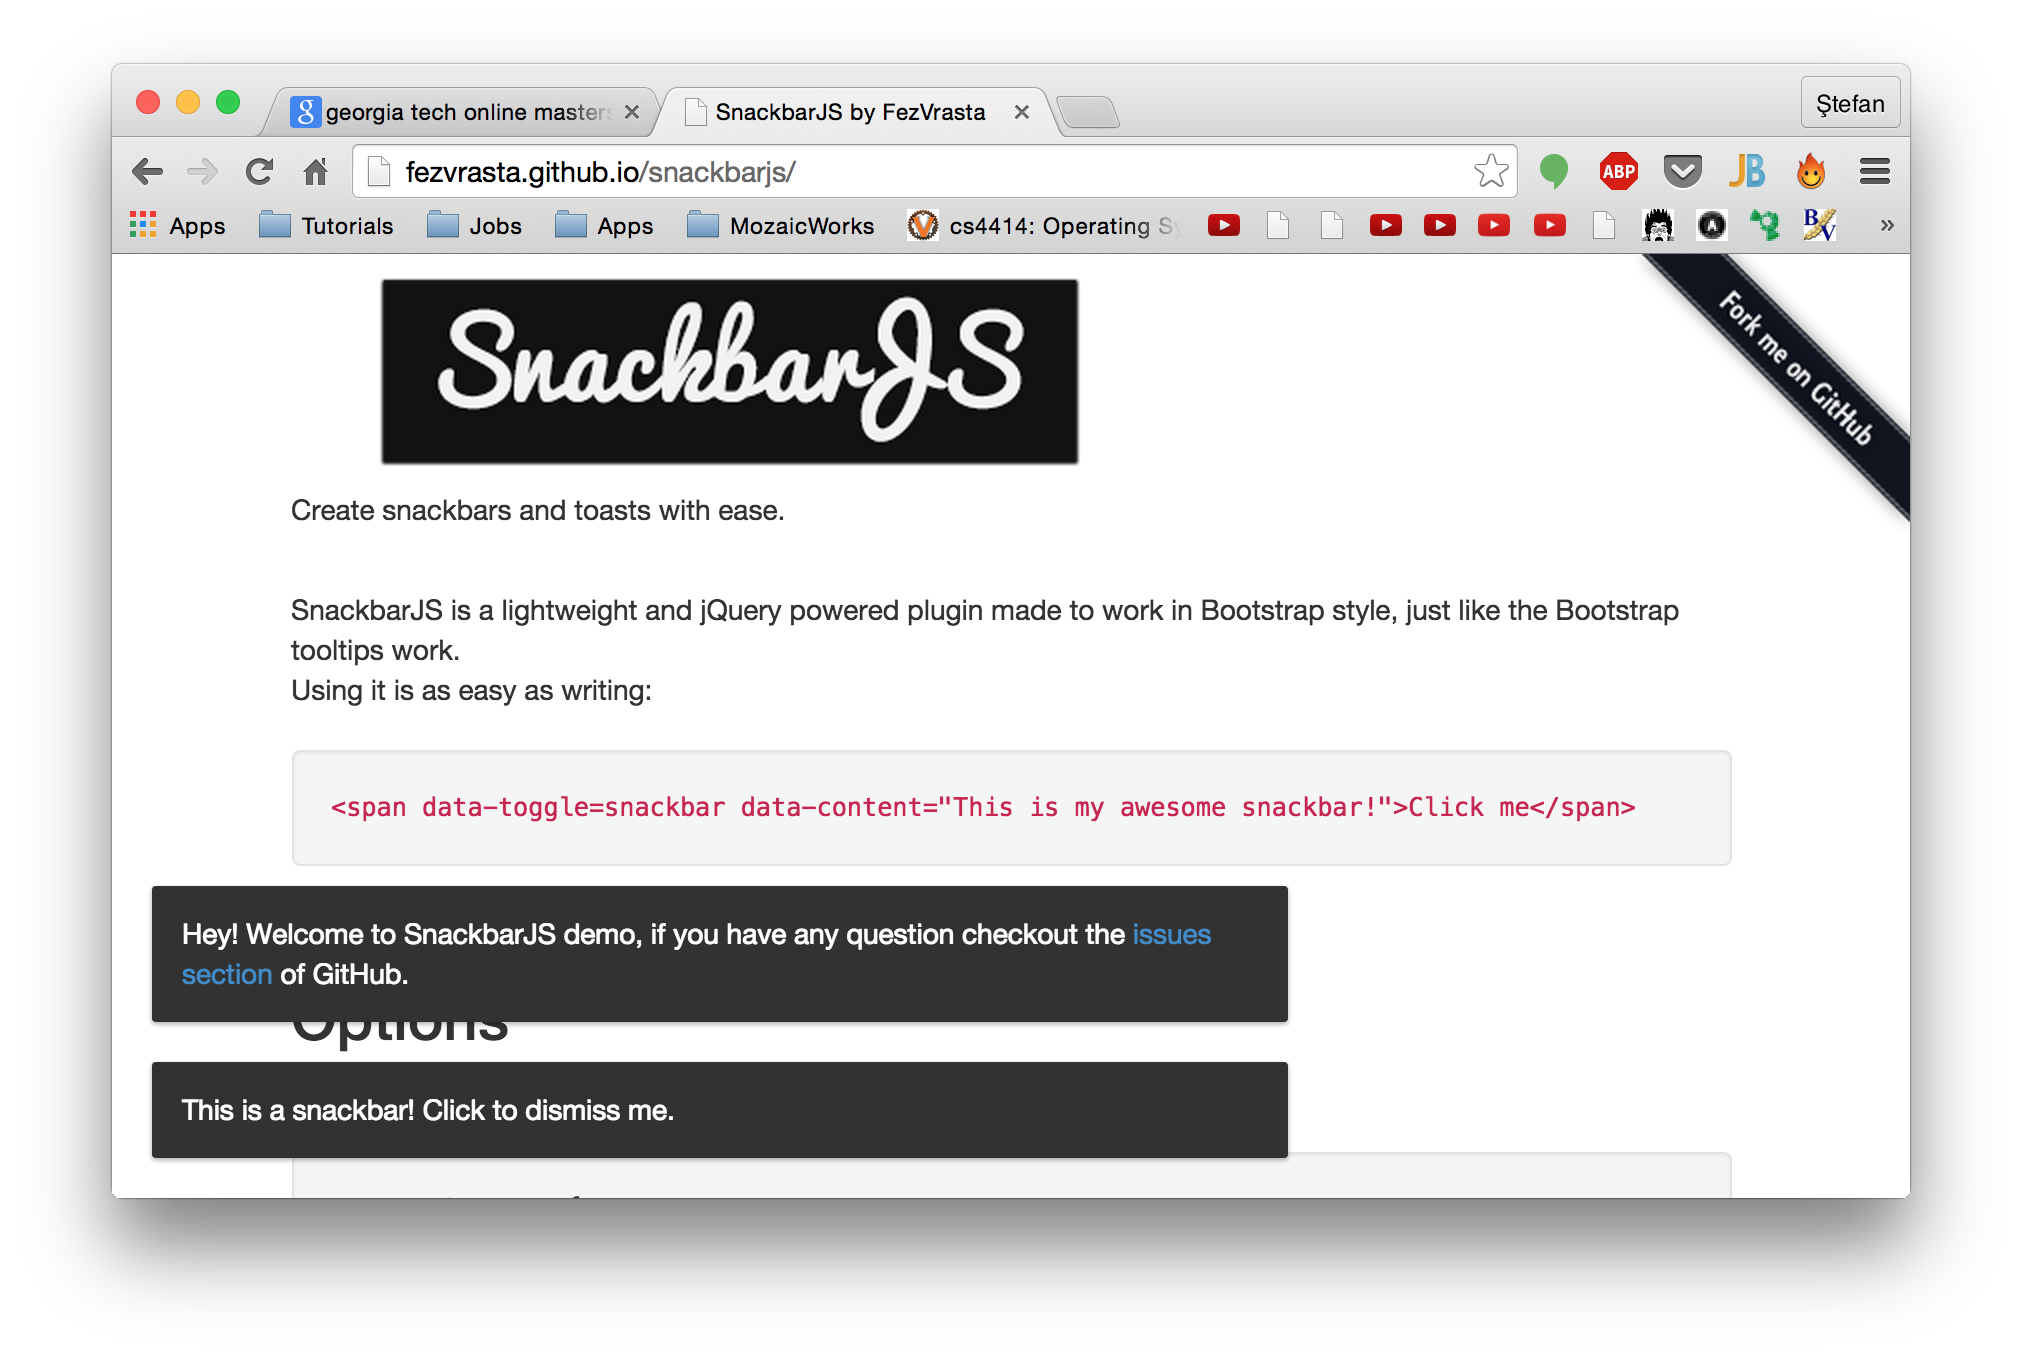
\includegraphics[width=1\textwidth]{./chap6-files/snackbar}
  \caption{Exemple de mesaje Snackbar de pe pagina librăriei javascript}
  \label{fig:snackbar}
\end{figure}

\lstinputlisting[title=static/js/utils/services/snackbar.service.js]{./chap6-files/snackbar.service.js}

\section{Posibilități de îmbunătățire ale aplicației}

Datorită limitărilor de timp, există numeroare posibilități de 
îmbunătățire și extindere a aplicației. De exemplu:
\begin{itemize}
\item Adăugare login cu Facebook. Acesta este așteptat de la
majoritatea aplicațiilor din ziua de azi, eliminând necesitatea
utilizatorului de a-și crea un cont pentru fiecare aplicație folosită.
\item Înlocuirea login-ului pe bază de cookie cu un alt mecanism,
de exemplu OAuth. Acest lucru decuplează back-end-ul de front-end, 
astfel API-ul REST ar putea fi folosit
și de aplicații mobile.
\item Îmbunătățirea stilurilor CSS.
\item Filtrarea pe server în loc de client.
\end{itemize}
